\documentclass[11pt, compress]{beamer}
\usepackage{amsmath}
\usetheme{Boadilla}
\usefonttheme[onlymath]{serif}
%get rid of navigation:
\setbeamertemplate{navigation symbols}{}


 %%%% Start PreTeXt generated preamble: %%%%% 

%% Some aspects of the preamble are conditional,
%% the LaTeX engine is one such determinant
\usepackage{ifthen}
\newcommand{\tabularfont}{}
\usepackage[xparse, raster]{tcolorbox}
\tcbset{colback=white, colframe=white}
\NewTColorBox{image}{mmm}{boxrule=0.25pt, colframe=gray, left skip=#1\linewidth,width=#2\linewidth}
\RenewTColorBox{definition}{m}{colback=teal!30!white, colbacktitle=teal!30!white, coltitle=black, colframe=gray, boxrule=0.5pt, sharp corners=downhill, titlerule = 0.25pt, title={#1}}
\RenewTColorBox{theorem}{m}{colback=pink!30!white, colbacktitle=pink!30!white, coltitle=black, colframe=gray, boxrule=0.5pt, sharp corners=downhill, titlerule = 0.25pt, title={#1}}
\RenewTColorBox{proof}{}{boxrule=0.25pt, colframe=gray, colback=white, before upper={Proof:}, after upper={\qed}}
%% tcolorbox styles for sidebyside layout
\tcbset{ bwminimalstyle/.style={size=minimal, boxrule=-0.3pt, frame empty,
colback=white, colbacktitle=white, coltitle=black, opacityfill=0.0} }
\tcbset{ sbsstyle/.style={raster before skip=2.0ex, raster equal height=rows, raster force size=false} }
\tcbset{ sbspanelstyle/.style={bwminimalstyle} }
%% Enviroments for side-by-side and components
%% Necessary to use \NewTColorBox for boxes of the panels
%% "newfloat" environment to squash page-breaks within a single sidebyside
%% "xparse" environment for entire sidebyside
\NewDocumentEnvironment{sidebyside}{mmmm}
  {\begin{tcbraster}
    [sbsstyle,raster columns=#1,
    raster left skip=#2\linewidth,raster right skip=#3\linewidth,raster column skip=#4\linewidth]}
  {\end{tcbraster}}
%% "tcolorbox" environment for a panel of sidebyside
\NewTColorBox{sbspanel}{mO{top}}{sbspanelstyle,width=#1\linewidth,valign=#2}
\newcommand{\lt}{<}
\newcommand{\gt}{>}
\newcommand{\amp}{&}

%% Begin: Semantic Macros
%% To preserve meaning in a LaTeX file
%%
%% \mono macro for content of "c", "cd", "tag", etc elements
%% Also used automatically in other constructions
%% Simply an alias for \texttt
%% Always defined, even if there is no need, or if a specific tt font is not loaded
\newcommand{\mono}[1]{\texttt{#1}}
%%
%% Following semantic macros are only defined here if their
%% use is required only in this specific document
%%
%% Used for inline definitions of terms
\newcommand{\terminology}[1]{\textbf{#1}}
%% End: Semantic Macros

\renewcommand{\d}{\displaystyle}
\newcommand{\N}{\mathbb N}
\newcommand{\B}{\mathbf B}
\newcommand{\Z}{\mathbb Z}
\newcommand{\Q}{\mathbb Q}
\newcommand{\R}{\mathbb R}
\def\C{\mathbb C}
\def\U{\mathcal U}
\newcommand{\pow}{\mathcal P}
\newcommand{\inv}{^{-1}}
\newcommand{\st}{:}
\renewcommand{\iff}{\leftrightarrow}
\newcommand{\Iff}{\Leftrightarrow}
\newcommand{\imp}{\rightarrow}
\newcommand{\Imp}{\Rightarrow}
\newcommand{\isom}{\cong}

\renewcommand{\bar}{\overline}
\newcommand{\card}[1]{\left| #1 \right|}
\newcommand{\twoline}[2]{\begin{pmatrix}#1 \\ #2 \end{pmatrix}}

\newcommand{\vtx}[2]{node[fill,circle,inner sep=0pt, minimum size=4pt,label=#1:#2]{}}
\newcommand{\va}[1]{\vtx{above}{#1}}
\newcommand{\vb}[1]{\vtx{below}{#1}}
\newcommand{\vr}[1]{\vtx{right}{#1}}
\newcommand{\vl}[1]{\vtx{left}{#1}}
\renewcommand{\v}{\vtx{above}{}}

%% Graphics Preamble Entries
\usepackage{tikz, pgfplots}

\usetikzlibrary{positioning,matrix,arrows}

\usetikzlibrary{shapes,decorations,shadows,fadings,patterns}
\usetikzlibrary{decorations.markings}

\usepackage{skak} %for chessboards etc.

\def\circleA{(-.5,0) circle (1)}
\def\circleAlabel{(-1.5,.6) node[above]{$A$}}
\def\circleB{(.5,0) circle (1)}
\def\circleBlabel{(1.5,.6) node[above]{$B$}}
\def\circleC{(0,-1) circle (1)}
\def\circleClabel{(.5,-2) node[right]{$C$}}
\def\twosetbox{(-2,-1.4) rectangle (2,1.4)}
\def\threesetbox{(-2.5,-2.4) rectangle (2.5,1.4)}
\newcommand{\hexbox}[3]{
  \def\x{-cos{30}*\r*#1+cos{30}*#2*\r*2}
  \def\y{-\r*#1-sin{30}*\r*#1}
  \draw (\x,\y) +(90:\r) -- +(30:\r) -- +(-30:\r) -- +(-90:\r) -- +(-150:\r) -- +(150:\r) -- cycle;
  \draw (\x,\y) node{#3};
}

\tikzset{->-/.style={decoration={
  markings,
  mark=at position .5 with {\arrow{>}}},postaction={decorate}}}

  \newcommand{\onedot}{
    +(.5,.5) \v
  }
  \newcommand{\twodots}{
    +(.25,.25) \v +(.75,.75) \v
  }
  \newcommand{\threedots}{
  +(.25,.25) \v +(.5, .5) \v +(.75,.75) \v
  }
  \newcommand{\fourdots}{
    +(.25,.25) \v +(.25,.75) \v +(.75,.25) \v +(.75,.75) \v
  }
  \newcommand{\fivedots}{
    +(.5,.5) \v +(.25,.25) \v +(.25,.75) \v +(.75,.25) \v +(.75,.75) \v
  }
  \newcommand{\sixdots}{
    +(.25,.5) \v +(.75,.5) \v +(.25,.25) \v +(.25,.75) \v +(.75,.25) \v +(.75,.75) \v
  }
  \newcommand{\dominoborder}{
    \draw[thick, rounded corners] (0,0) rectangle (1,2);
    \draw[thin] (0,1) -- (1,1);
  }


%%%% End of PreTeXt generated preamble %%%%% 

\title{Arithmetic and Geometric Sequences}
\subtitle{(Section 2.2)}
\author{}
\date[]{}

\begin{document}
\begin{frame}
\maketitle 
\end{frame}
 
\begin{frame}
\frametitle{Overview}
\tableofcontents 
\end{frame}
 

\section{Arithmetic and Geometric Sequences}
\begin{frame}
\frametitle{Investigate!}
 For the patterns of dots below, draw the next pattern in the sequence. Then give a recursive definition and a closed formula for the number of dots in the \(n\)th pattern.
 \begin{sidebyside}{1}{0.175}{0.175}{0}%
\begin{sbspanel}{0.65}%
\resizebox{\linewidth}{!}{%
        \begin{tikzpicture}
\draw[fill = black] (0,0) \v;
\node[below] at (0,-.6) {$n = 0$};

  \draw[fill = black] (0+3,0) \v (.3+3, .3) \v (-.3+3,-.3) \v (-.3+3, .3) \v (.3+3,-.3) \v;
    \node[below] at (0+3,-.6) {$n = 1$};

  \draw[fill = black] (0+6,0) \v (.3+6, .3) \v (-.3+6,-.3) \v (-.3+6, .3) \v (.3+6,-.3) \v (.6+6, .6) \v (-.6+6,-.6) \v (-.6+6, .6) \v (.6+6,-.6) \v;
    \node[below] at (0+6,-.6) {$n = 2$};
  \end{tikzpicture}
}%
\end{sbspanel}%
\end{sidebyside}%
 \begin{sidebyside}{1}{0.175}{0.175}{0}%
\begin{sbspanel}{0.65}%
\resizebox{\linewidth}{!}{%
        \begin{tikzpicture}
\draw[fill = black] (0,.25) \v (0,-.25) \v;
\node[below] at (0,-1.5) {$n = 0$};

  \draw[fill = black] (-.5+3,.25) \v (.5+3, .25) \v (0+3, .95) \v (-.5+3,-.25) \v (.5+3, -.25) \v (0+3,-.95) \v;
  \node[below] at (0+3,-1.5) {$n = 1$};

  \draw[fill = black] (-.7+6,.25) \v (-.3+6,.25) \v (-.5+6,.6) \v
  	(.3+6, .25) \v (.7+6,.25) \v (.5+6, .6) \v
  	(-.2+6, .95) \v (.2+6, .95) \v (0+6, 1.3) \v
    (-.7+6,-.25) \v (-.3+6,-.25) \v (-.5+6,-.6) \v
      (.3+6, -.25) \v (.7+6,-.25) \v (.5+6, -.6) \v
      (-.2+6, -.95) \v (.2+6, -.95) \v (0+6, -1.3) \v;
    \node[below] at (0+6,-1.5) {$n = 2$};
  \end{tikzpicture}
}%
\end{sbspanel}%
\end{sidebyside}%
 \begin{sidebyside}{1}{0.15}{0.15}{0}%
\begin{sbspanel}{0.7}%
\resizebox{\linewidth}{!}{%
        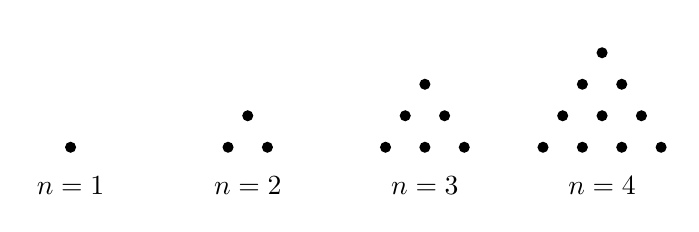
\begin{tikzpicture}
\draw[fill = black] (0,0) \v;
\node[below] at (0,-.25) {$n = 1$};

  \draw[fill = black] (0+2,0) \v (.5+2, 0) \v (.25+2,.4) \v;
  \node[below] at (.25+2,-.25) {$n = 2$};

  \draw[fill = black] (0+4,0) \v (.5+4, 0) \v (.25+4,.4) \v (1+4,0) \v (.75+4,.4) \v (.5+4, .8) \v;
  \node[below] at (.5+4,-.25) {$n = 3$};

      \draw[fill = black] (0+6,0) \v (.5+6, 0) \v (.25+6,.4) \v (1+6,0) \v (.75+6,.4) \v (.5+6, .8) \v (1.5+6, 0) \v (1.25+6, .4) \v (1+6, .8) \v (.75+6, 1.2) \v;
      \node[below] at (.75+6,-.25) {$n = 4$};
      \end{tikzpicture}
}%
\end{sbspanel}%
\end{sidebyside}%
\end{frame}
 
\begin{frame}
\frametitle{Arithmetic Sequences}
 If the terms of a sequence differ by a constant, we say the sequence is \terminology{arithmetic}. \index{arithmetic sequence} If the initial term (\(a_0\)) of the sequence is \(a\) and the \terminology{common difference} is \(d\), then we have,
 Recursive definition: \(a_n = a_{n-1} + d\) with \(a_0 = a\).
 Closed formula: \(a_n = a + dn\).
\end{frame}
 
\begin{frame}
\frametitle{}
\begin{example}[2.2.1]Find recursive definitions and closed formulas for the arithmetic sequences below. Assume the first term listed is \(a_0\).
\begin{enumerate}
\item{} \(2, 5, 8, 11, 14, \ldots\).

\item{} \(50, 43, 36, 29, \ldots\).
\end{enumerate}

\end{example}
\end{frame}
 
\begin{frame}
\frametitle{Geometric Sequences}
 A sequence is called \terminology{geometric} \index{geometric sequence} if the ratio between successive terms is constant. Suppose the initial term \(a_0\) is \(a\) and the \terminology{common ratio} is \(r\). Then we have,
 Recursive definition: \(a_n = ra_{n-1}\) with \(a_0 = a\).
 Closed formula: \(a_n = a\cdot r^{n}\).
\end{frame}
 
\begin{frame}
\frametitle{}
\begin{example}[2.2.2]Find the recursive and closed formula for the geometric sequences below. Again, the first term listed is \(a_0\).\begin{enumerate}
\item{} \(\displaystyle 3, 6, 12, 24, 48, \ldots\)

\item{} \(\displaystyle 27, 9, 3, 1, 1/3, \ldots\)
\end{enumerate}

\end{example}
\end{frame}
 


\section{Sums of Arithmetic and Geometric Sequences}
\begin{frame}
\frametitle{Investigate!}
 Your neighborhood grocery store has a candy machine full of Skittles.\begin{enumerate}
\item{} Suppose that the candy machine currently holds exactly 650 Skittles, and every time someone inserts a quarter, exactly 7 Skittles come out of the machine.\begin{enumerate}
\item{} How many Skittles will be left in the machine after 20 quarters have been inserted?


\item{} Will there ever be exactly zero Skittles left in the machine? Explain.

\end{enumerate}



\item{} What if the candy machine gives 7 Skittles to the first customer who put in a quarter, 10 to the second, 13 to the third, 16 to the fourth, etc. How many Skittles has the machine given out after 20 quarters are put into the machine?


\item{} Now, what if the machine gives 4 Skittles to the first customer, 7 to the second, 12 to the third, 19 to the fourth, etc. How many Skittles has the machine given out after 20 quarters are put into the machine?

\end{enumerate}

\end{frame}
 
\begin{frame}
\frametitle{}
\begin{example}[2.2.4]Find the sum: \(2 + 5 + 8 + 11 + 14 + \cdots + 470\).
\end{example}
\end{frame}
 
\begin{frame}
\frametitle{}
\begin{example}[2.2.5]Find a closed formula for \(6 + 10 + 14 + \cdots + (4n - 2)\).
\end{example}
\end{frame}
 
\begin{frame}
\frametitle{}
\begin{example}[2.2.6]Use partial sums to find a closed formula for \((a_n)_{n\ge 0}\) which starts \(2, 3, 7, 14, 24, 37,\ldots \ldots\)
\end{example}
\end{frame}
 
\begin{frame}
\frametitle{}
\begin{example}[2.2.7]What is \(3 + 6 + 12 + 24 + \cdots + 12288\)?
\end{example}
\end{frame}
 
\begin{frame}
\frametitle{}
\begin{example}[2.2.8]Find a closed formula for \(S(n) = 2 + 10 + 50 + \cdots + 2\cdot 5^n\).
\end{example}
\end{frame}
 
\begin{frame}
\frametitle{}
\begin{example}[2.2.9]Express \(0.464646\ldots\) as a fraction.
\end{example}
\end{frame}
 

\end{document}
